\documentclass[../../thesis.tex]{subfiles}
\graphicspath{{\subfix{../../resources/}}}
\begin{document}

\section{Results}
In this section, all results to answer our research questions are visualised and 
discussed in \autoref{sec:evaluation:interpretation}.


% \subsection{Group Sampling}
% \subsection{Real world datasets}
\begin{figure}[!htbp]
    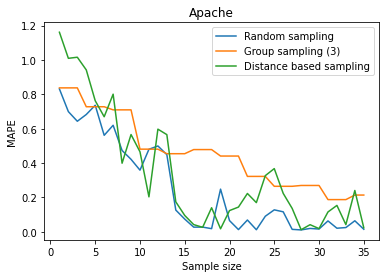
\includegraphics[width=0.5\textwidth]{graphs/apache_group_vs_random_sampling.png}
    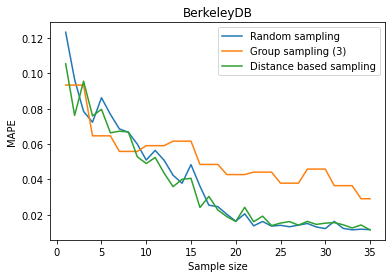
\includegraphics[width=0.5\textwidth]{graphs/berkley_group_vs_random_sampling.png}
    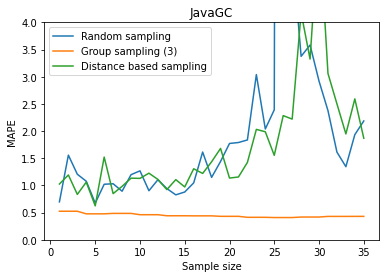
\includegraphics[width=0.5\textwidth]{graphs/javagc_group_vs_random_sampling.png} 
    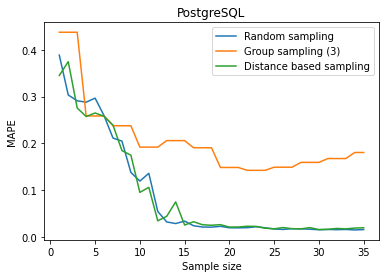
\includegraphics[width=0.5\textwidth]{graphs/postgre_group_vs_random_sampling.png}
    \caption[Group sampling and random sampling on real world examples]{
        Group Sampling compared to random sampling with linear regression on real world examples
    }\label{fig:evaluation:mape_real}
\end{figure}

% \subsection{Large datasets}
\begin{figure}[!htbp]
    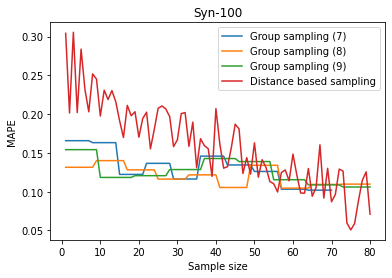
\includegraphics[width=0.5\textwidth]{graphs/syn-100_gs_7_8_9_vs_distance.png}
    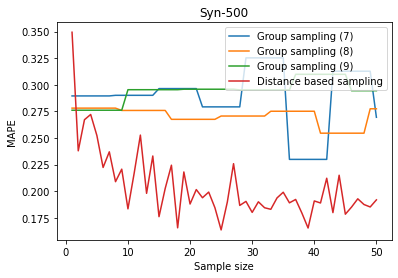
\includegraphics[width=0.5\textwidth]{graphs/syn-500_gs_7_8_9_vs_distance.png}
    \begin{center}
        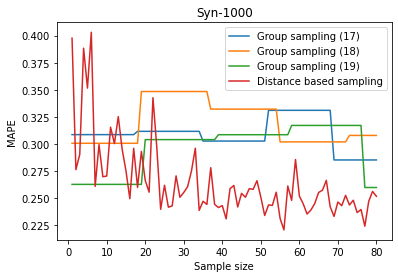
\includegraphics[width=0.5\textwidth]{graphs/syn-1000_gs_17_18_19_vs_distance.png}
    \end{center}
    \caption[Group sampling and random sampling on synthetic datasets]{
        Group sampling compared to distance based sampling with linear regression on synthetic data.
    }\label{fig:evaluation:mape_syn}
\end{figure}




% \subsection{Feature interactions}
\begin{figure}[!htbp]
    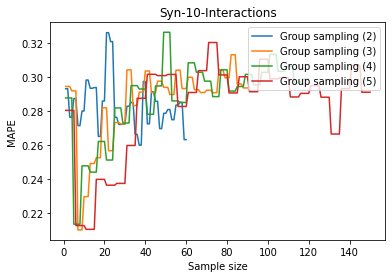
\includegraphics[width=0.5\textwidth]{graphs/syn-10-int-mape.png}
    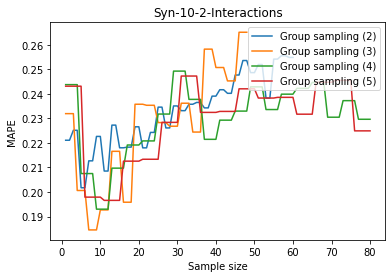
\includegraphics[width=0.5\textwidth]{graphs/syn-10-2-int-mape.png}
    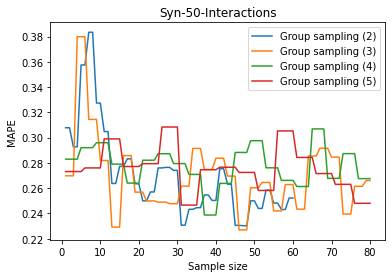
\includegraphics[width=0.5\textwidth]{graphs/syn-50-int-mape.png}
    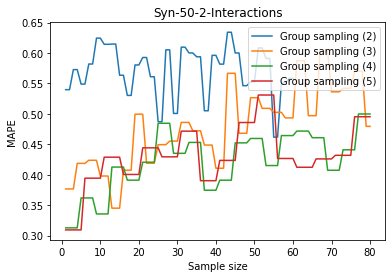
\includegraphics[width=0.5\textwidth]{graphs/syn-50-2-int-mape.png}
    \caption[Group sampling with feature interactions]{
        Group sampling with feature interactions
    }\label{fig:evaluation:interactions}
\end{figure}

\FloatBarrier


\end{document}